\section*{Appendices}
\begin{appendices}
	
	\section{Robot energy consumption calculation}\label{sec:app_robot_ener_consumption}
	
	
\begin{figure}[!t]
	\centering
	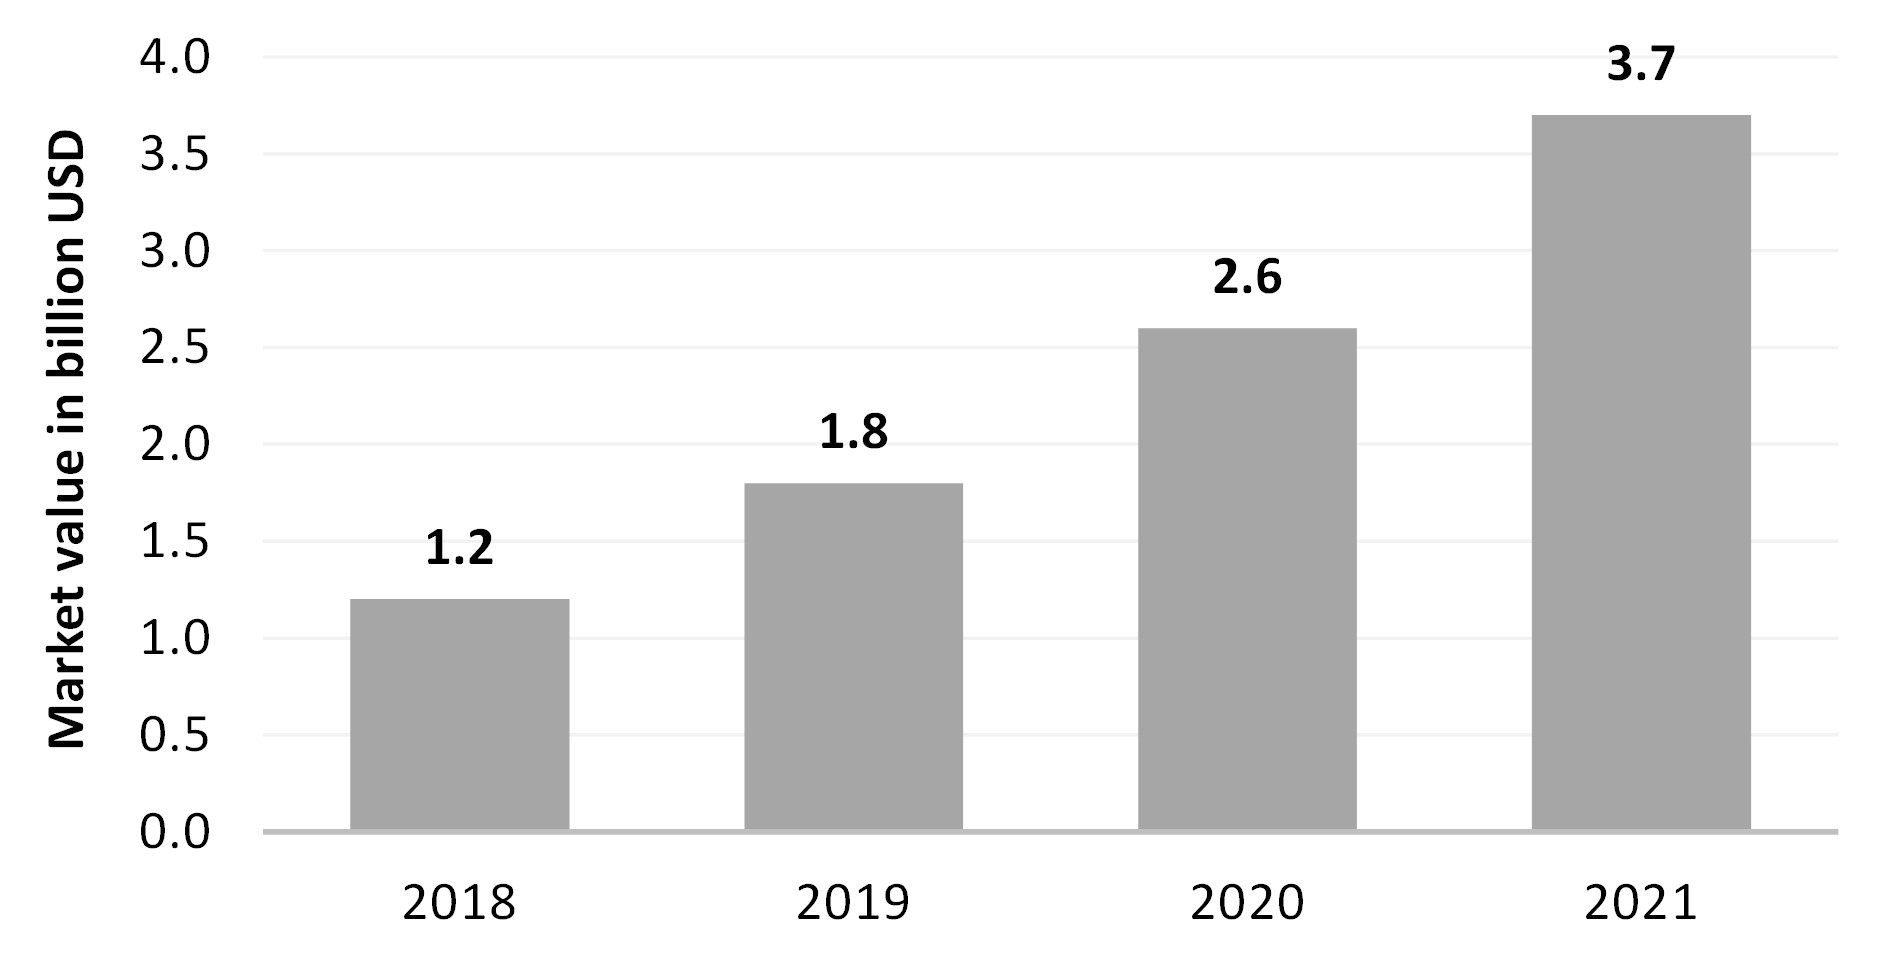
\includegraphics[width= 0.9\columnwidth]{fig/advanced_robots_in_manufacturing_projected_global_demand}
	\caption{Projected demand for advanced robotics in manufacturing worldwide between 2018 and 2021 (in billion USD).}
	\label{fig:advanced_robots_in_manufacturing_projected_global_demand}
\end{figure}	
	
	According to \cite{montaqim2015}, and available press releases of different robotic companies (\cite{fanuc2015, yaskawa2014, ABB2015}), the current distribution of the install base per manufacturer is shown in figure \ref{fig:manufacturers_pie}.
	%---
	\begin{figure}[!ht]
		\centering
		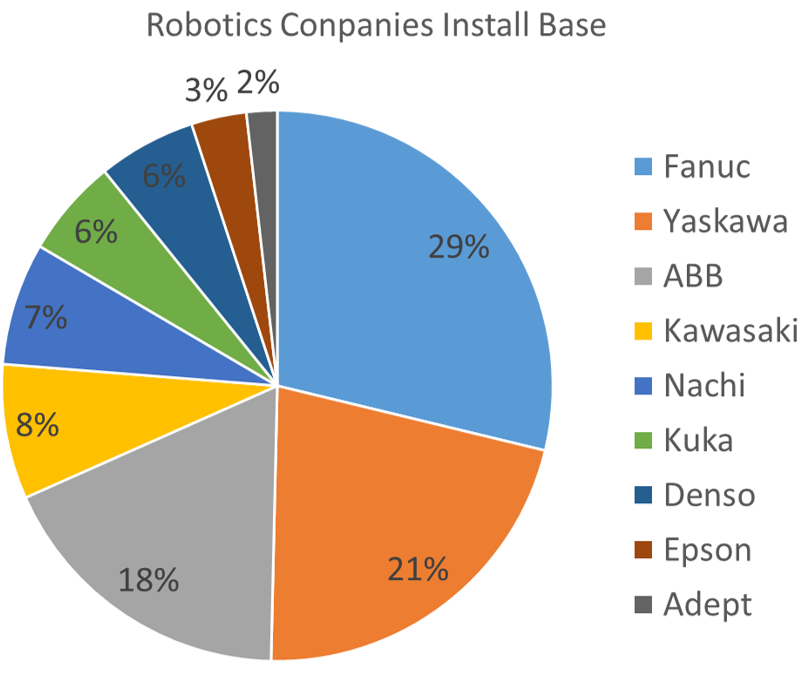
\includegraphics[width=0.4\textwidth]{fig/manufacturers}
		\caption{Percentage of installed robots per manufacturer}
		\label{fig:manufacturers_pie}
	\end{figure}
	%---
	Figure \ref{fig:manufacturers} shows that Fanuc, Yaskawa, and ABB comprise 68\% of the total install base of industrial robots in the world \textcolor{red}{\textbf{NEEDS UPDATE!!!}}. Thus, it was decided to take these three companies as a representative sample to estimate the total power consumption. The datasheets for their robot portfolio were surveyed in order to find the average power consumption for each model. Additionally, every manufacturer classifies their robots according to one or more possible applications which can be grouped into the application categories defined by the IFR. For every application, the average power consumption was calculated using the values reported in the robot datasheets. Finally, the power consumption for each category was computed as a weighted average based on the companies' market share percentage (assuming that the 68\% is the total number of robots)\footnote[1]{These numbers should be used with discretion since there is no available information on which are the most common installed robot models. This information may change the estimation.} The estimated power consumption per robot application is shown in figure \ref{fig:average_power}.
	%---
	\begin{figure}[h]
		\centering
		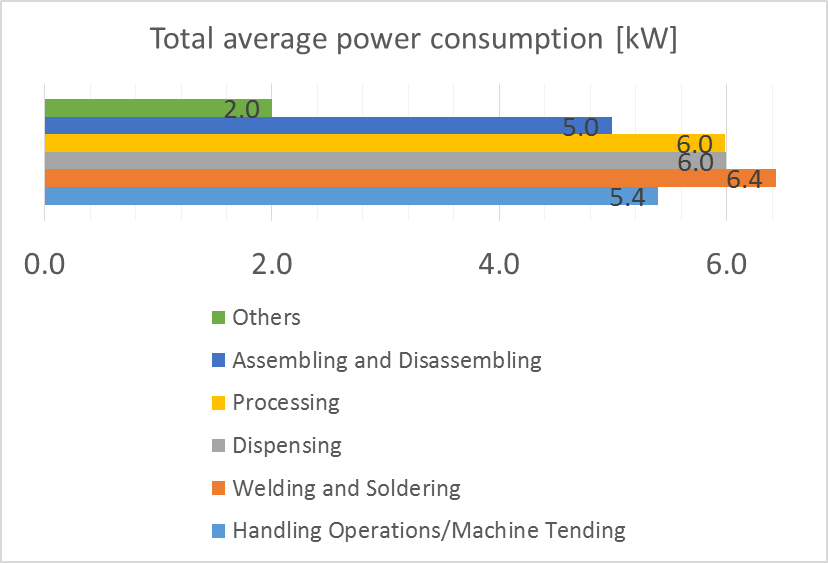
\includegraphics[width=0.45\textwidth]{fig/average_power}
		\caption{Average power consumption per category}
		\label{fig:average_power}
	\end{figure}
	%---
	\section{Collaborative robots}
	Information taken from \url{https://www.statista.com/statistics/748128/estimated-collaborative-robot-sales-worldwide/}
	\begin{figure}[!ht]
		\centering
		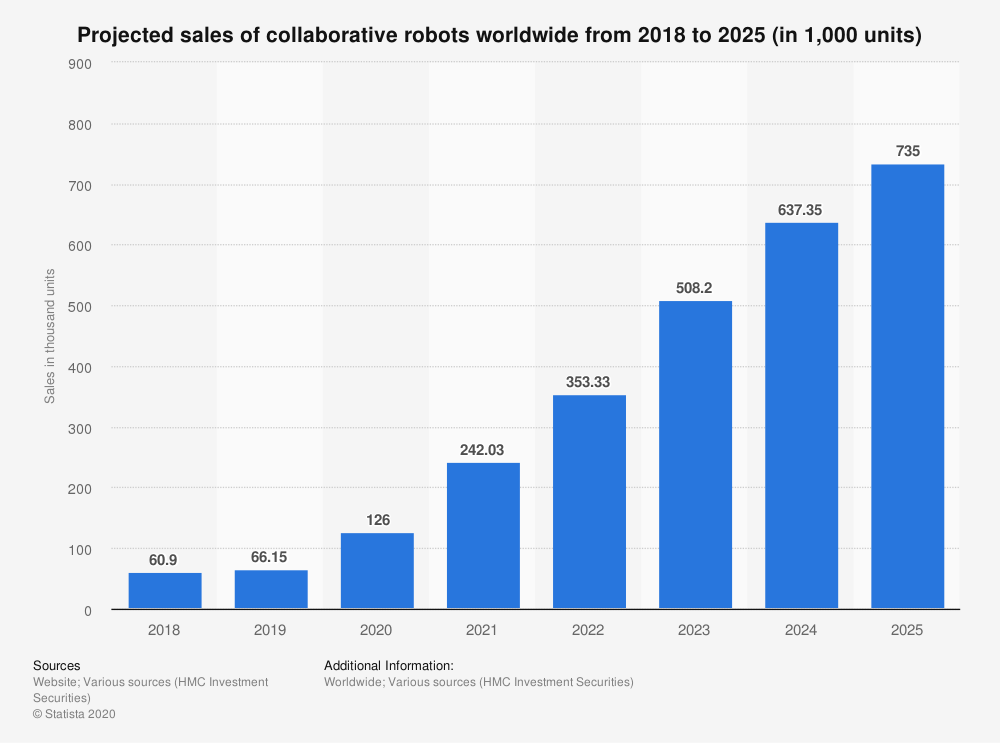
\includegraphics[width=0.4\textwidth]{fig/cobots_global_sales_2018_2025}
		\caption{Projected sales of collaborative robots worldwide from 2018 to 2025 (in 1,000 units)}
		\label{fig:cobots_sales_projection}
	\end{figure}
	
	Taken from \url{https://www.statista.com/statistics/1044767/collaborative-robots-market-by-application/}
	\begin{figure}[!ht]
		\centering
		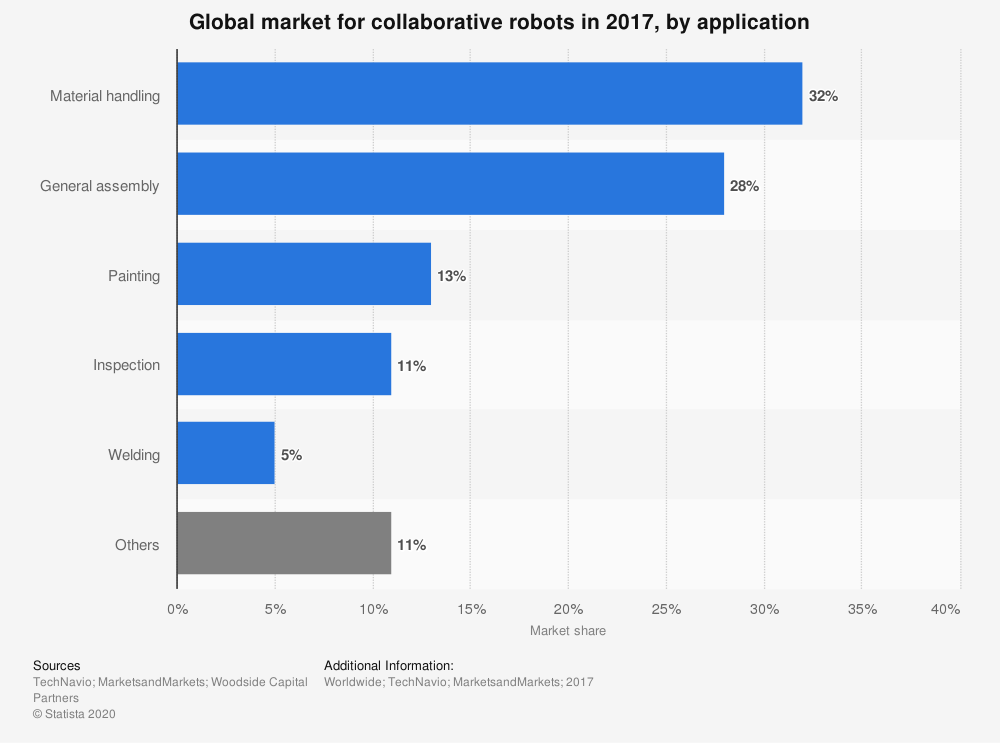
\includegraphics[width=0.4\textwidth]{fig/global_market_size_cobots_by_application}
		\caption{Global market for collaborative robots in 2017, by application.}
		\label{fig:global_market_size_cobots_by_application}
	\end{figure}
	
	\section{Service robots}
	\begin{figure}[h]
		\centering
		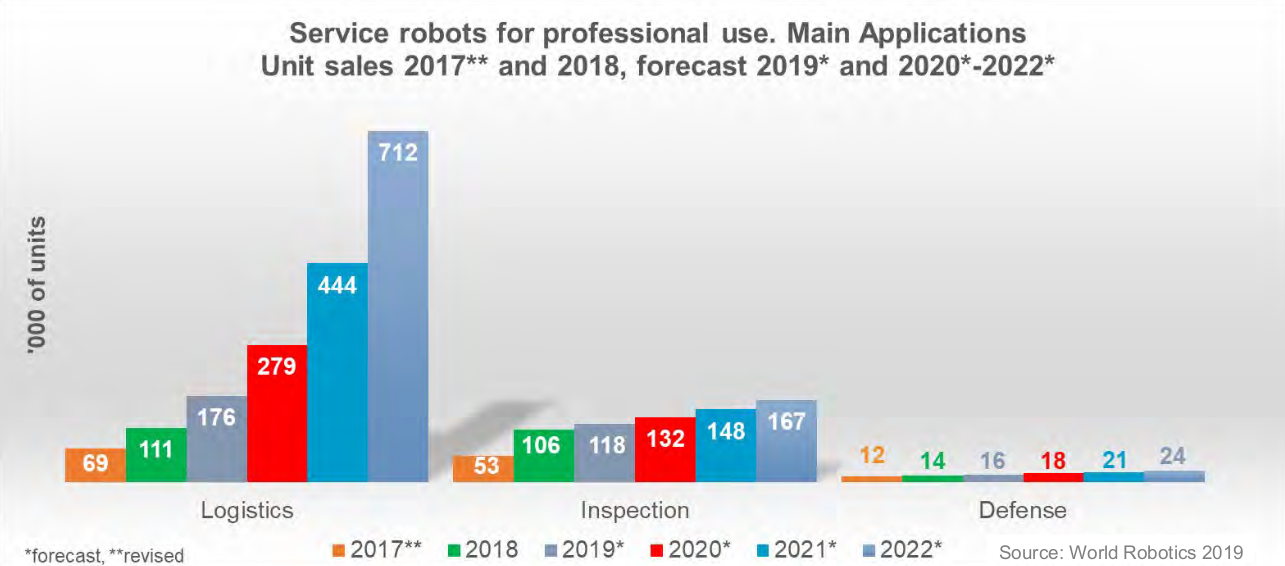
\includegraphics[width=0.4\textwidth]{fig/service_robots_professional_use_main_app_sales}
		\caption{Unit sales of service robots for professional use.}
		\label{fig:service_robots_professional_use_main_app_sales}
	\end{figure}
	
	\begin{figure}[h]
		\centering
		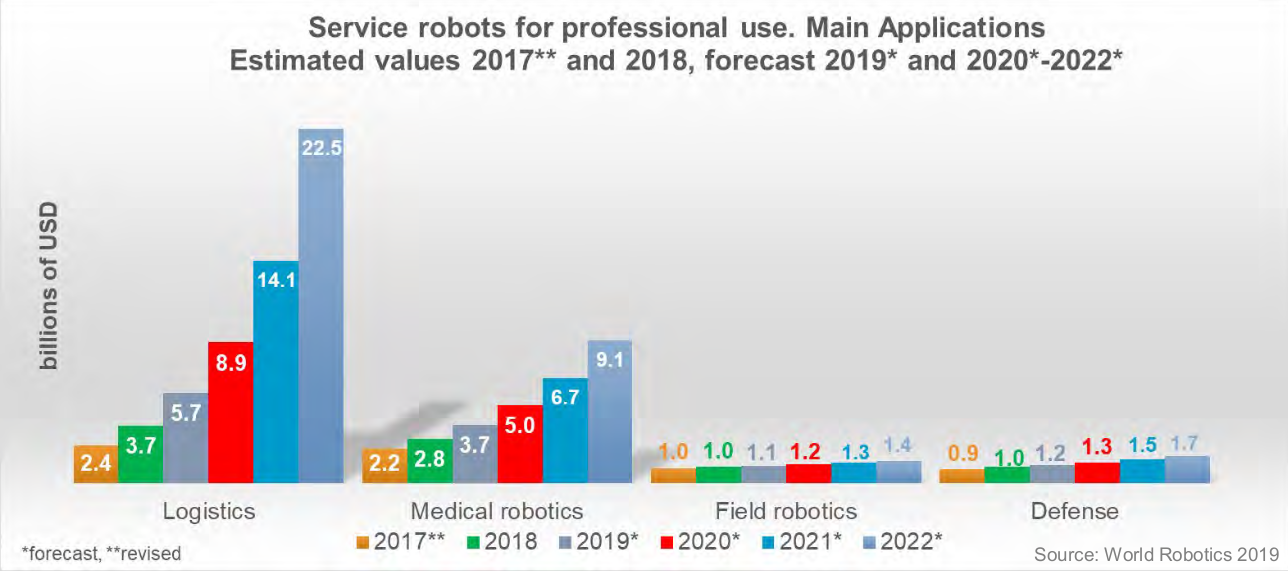
\includegraphics[width=0.4\textwidth]{fig/service_robots_professional_main_app_value}
		\caption{Estimated market value of service robots for professional use according to their main application.}
		\label{fig:service_robots_professional_main_app_value}
	\end{figure}
	
	\begin{figure}[h]
		\centering
		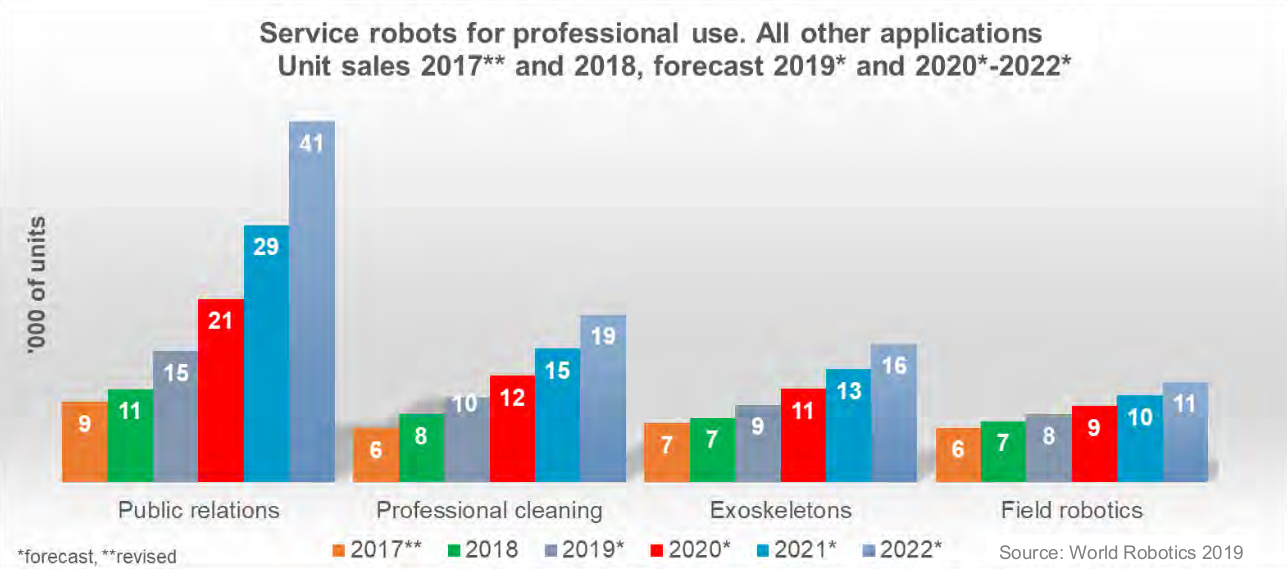
\includegraphics[width=0.4\textwidth]{fig/service_robots_professional_use_main_other_sales}
		\caption{Unit sales for service robots for other professional use.}
		\label{fig:service_robots_professional_use_main_other_sales}
	\end{figure}
	
	
\end{appendices}

% Notes:
% Up to now: Time is saved by increasing resources (more computation power, means faster)
% This ultimately leads to disaster (the energy is simply not there)
% It is not enough to reduce the individual energy consumption
% Solution to systematically and independent of the particular technology to reduce both energy and time at the same time is collective learning based on transfer learning

% Task energy cannot be reduced. The body needs that energy times efficiency. Even if efficiency is 1 -> too many tasks -> too much energy
% Thought experiment
% Learning needs a lot of energy (executing and computing)
% Relevance

% Deprecated introduction: